\PassOptionsToPackage{top=3cm,left=3cm,right=3cm,bottom=3cm}{geometry}
\documentclass[fleqn,11pt]{wlscirep}

\usepackage{import}
\usepackage{main}

\renewcommand{\paragraph}[1]{\vspace{0.3cm}\noindent\underline{\emph{#1}}\hfill\noindent}

% word count
% \newcommand{\maincount}[1]{%
%   \immediate\write18{texcount -1 -sum=1 -merge -q -nobib #1.tex > #1-words.sum}%
%   \input{#1-words.sum}%
% }

% \newcommand{\abstractcount}[1]{%
%   \immediate\write18{texcount -template="{abst}" #1.tex > #1-words.sum}%
%   \input{#1-words.sum}%
% }

\begin{document}

\doublespacing

\title{\bfseries\LARGE\singlespacing{A novel spatiotemporal model to estimate \emph{Mycobacterium} tuberculosis transmission risks in crowded indoor settings using environmental, clinical, and patient movement data}}
% author list
\author[1]{Nicolas Banholzer}
\author[2]{Keren Middelkoop}
\author[2]{Juane Leukes}
\author[3]{Ernest Weingartner}
\author[1]{Remo Schmutz}
\author[1]{Kathrin Zürcher}
\author[1]{Matthias Egger}
\author[2]{Robin Wood}
\author[1*]{Lukas Fenner}

\affil[1]{Institute of Social and Preventive Medicine, University of Bern, Bern, Switzerland}
\affil[2]{Desmond Tutu HIV Centre, Department of Medicine, University of Cape Town, Cape Town, South Africa}
\affil[3]{Institute for Sensors and Electronics, University of Applied Sciences and Arts Northwestern Switzerland, Windisch, Switzerland}

\affil[*]{Corresponding author: lukas.fenner@unibe.ch }

\vspace{1em}

% \begin{information}\normalfont
% \noindent\textbf{Running head}: SARS-COV-2 transmission in schools and effect of air cleaners

% %\noindent\textbf{Subject categorization}: 6.20  Indoor Air; 10.11 Pediatrics: Respiratory Infections

% \noindent\textbf{Word count}: \maincount{manuscript}words, abstract \abstractcount{manuscript}words (max. 500), title 157 chars (max. 200)

% %\noindent\textbf{Inserts:} 2 tables, 6 figures, 44 references

% \noindent\textbf{S1 Appendix:} Includes supplementary text, tables and figures.

% \vspace{1em}

% \noindent\textbf{Funding}

% \noindent This study is funded by the Multidisciplinary Center for Infectious Diseases, University of Bern, Bern, Switzerland. NB, LF, and ME are supported by the National Institute of Allergy and Infectious Diseases (NIAID) through cooperative agreement 5U01-AI069924-05. ME is supported by special project funding from the Swiss National Science Foundation (grant 32FP30-189498). \medskip

% \noindent\textbf{Contributions}

% \noindent Conception and design: NB, LF. Epidemiological and environmental data collection: NB, PJ, TS, LF. Laboratory data collection: PB, LFu. Additional data collection: TH. Statistical analysis: NB, KZ. Genomic analysis: LB, LFu. Paper draft: NB, LF, ME. All authors reviewed and approved the final version of the manuscript.

% \par
% \end{information}

%TC:newcounter abst Words in abstract
%TC:envir abstract [] abst
\begin{abstract}\normalfont
\noindent\textbf{Background:} Tuberculosis (TB) caused by \emph{Mycobacterium tuberculosis (Mtb)} is strictly airborne and thus the risk of transmission is higher in crowded indoor environments, especially healthcare facilities. Existing approaches to modeling the risk of airborne transmission typically assume that the airspace is well mixed, not considering that proximity to infectious individuals may increase the risk of transmission. We aimed to develop a  spatiotemporal model of airborne \emph{Mtb} transmission using environmental, clinical, and patient movement data to estimate TB transmission during the COVID-19 pandemic in healthcare facilities and to evaluate the impact of infection control measures.

\noindent\textbf{Methods:} We collected environmental (CO$_2$ levels), clinical (patient visits and TB disease status), and patient movement data (anonymous patient tracking from video sensors) in a primary care clinic in Cape Town, South Africa, for five days in October/November 2021 during the COVID-19 pandemic when universal use of masks was compulsory and ventilation was increased. We matched patient movements with clinical records to identify the spatiotemporal location of  infectious TB patients. We modeled the spatiotemporal concentration of infectious doses (quanta) and estimated the patient-specific risk of infection using the Wells-Riley equation.

\noindent\textbf{Results:} Clinical records registered 894 patients, four of whom were diagnosed with TB. Video sensors detected 1,438 clinic attendees with a median stay of 25\,min (interquartile range [IQR] 13\,min$-$46\,min). CO$_2$ levels were low (median 431\,ppm, IQR 406\,ppm$-$458\,ppm), compatible with high ventilation rates. The modeled risk of infection per clinic attendee was 0.059\% (95\%-credible interval [CrI] 0.001\%$-$0.402\%). The risk would have increased 1.28-fold (95\%-CrI 1.19$-$1.36) without mask use and 1.74-fold (95\%-CrI 0.47$-$5.34) with lower, pre-pandemic ventilation rates. Furthermore, the individual risk was significantly associated with the number of close-contact encounters and time spent in the clinic. 

\noindent\textbf{Conclusions:} Our novel spatiotemporal transmission model estimated the risk of \emph{Mtb} transmission in a South African clinic as low during the COVID-19 pandemic, mainly due to infection control measures. Our spatiotemporal modeling could be used to identify high-risk areas and evaluate the impact of infection control measures in clinics. 

\par
\end{abstract}

%TC:ignore

\flushbottom
\maketitle
\setcounter{page}{1}
\thispagestyle{fancy}

\vspace{2em}

%\noindent\textbf{Word count:} \abstractcount{manuscript}words (max. 500)

\vspace{0.5em}

\noindent\textbf{Keywords:} Mycobacterium tuberculosis, airborne infection, patient tracking, spatiotemporal model
% maximum of 3-5 keywords
\newpage

\sloppy
\raggedbottom
%TC:endignore

\newpage

%TC:break main
\section{Introduction} 

% TB and the route of transmission
Tuberculosis (TB) is one of the leading causes of death worldwide, especially in the South African region, which is disproportionately affected by the TB burden. After two years of COVID-19-related disruption in the progress made in TB prevention and control before the pandemic, the impact of the pandemic is about to reverse \cite{WHO2022TBReport}. However, global TB targets have 
been largely missed (REF).  \emph{Mycobacterium tuberculosis} (\emph{Mtb}), the causative agent of TB, is transmitted via respiratory particles in the exhaled air of infectious persons\cite{Rieder1999,Patterson2021Tuberculosis}. \emph{Mtb} is primarily carried in smaller particles in the size range of $1-7\mu$m\cite{Fennelly2020Lancet}, which can survive in the air for multiple hours\cite{Loudon1969AMRRD}. Survival of airborne pathogens is greater in crowded, poorly ventilated indoor environments\cite{Rieder1999,CPS2013Book,Nardell1991ARRD,Wang2021Science,Morawska2021}. As such, healthcare facilities present a particularly high-risk setting because both more infectious and more susceptible individuals are also more likely to visit a clinic\cite{McCreesh2020IJTLD}. A modeling study in South Africa estimated that 4\% to 14\% of adult TB cases originate from primary care clinics\cite{McCreesh2022BMJGlobalHealth}.

% the Wells-Riley model and its limitations
The Wells-Riley model\cite{Riley1978AJE} is widely used to estimate the risk of airborne transmission in a variety of indoor settings\cite{Andrews2014JID,Taylor2016IJTLD,Hella2017JInfect,Zemouri2020JDR}, including primary care clinics\cite{Zurcher2022JID,McCreesh2021BMJGlobalHealth}. The model estimates the risk of infection based on the number of infectious individuals in space, the generation rate of infectious quanta (doses of pathogen-carrying particles), the breathing rate per person, and the outdoor air supply rate. The Wells-Riley model, and variations thereof\cite{Rudnick2003IndoorAir}, assume a well-mixed airspace, which means that the quanta concentration is the same throughout the room. However, the quanta concentration is typically higher near the infectious source\cite{Wang2021Science,Vuorinen2020SafSci,Chen2020BuildEnv}, and previous studies have shown that the risk of TB infection is associated with proximity to these individuals\cite{Ko2004RiskAnal,Kenyon1996NEJM}.

% what this study adds
We developed a spatiotemporal extension of the Wells-Riley model to model the concentration of infectious quanta in space and time. We combined clinical and person tracking data to determine the spatiotemporal location of TB patients and susceptible attendees at a primary care clinic in South Africa for five days in October/November 2021. We also measured indoor CO$_2$ levels to model the spatial diffusion and removal of infectious quanta over time. We used Monte Carlo simulation to estimate the risk of infection per clinic attendee. Finally, we assessed the impact of infection control measures in place during the study in response to the COVID-19 pandemic (mask use and increased ventilation) by modeling the risk of infection under hypothetical pre-pandemic scenarios without universal mask use and pre-pandemic ventilation conditions in the clinic.

\newpage

\section{Methods}

\subsection{Study design}

We build on the design of a pilot study in 2019\cite{Zurcher2022JID}, which was described in detail in a study protocol \cite{Zurcher2020BMJ}. We collected environmental data (indoor CO$_2$ levels), clinical data (TB status), and video sensor data (patient movements) for five days during the COVID-19 pandemic in October/November 2021 (October 13, 15, 25, and November 4, 5) at a primary care clinic in Cape Town, South Africa. 

\subsection{Study setting}

The primary care clinic offers both TB and HIV services as well as other basic clinical services, Monday through Friday, from 8\,am to 4\,pm. The clinic is located in a large settlement of formal and semi-formal housing where TB and HIV are highly prevalent\cite{Wood2007AMJRCCD,Middelkoop2011JAIDS}. We defined three areas within the clinic (\Cref{fig:floor-plan}): the waiting room (10.55m $\times$ 5.50m $\times$ 3.00m), corridor (12.45m $\times$ 2.20m $\times$ 2.50m), and TB room (4.75m $\times$ 3.50m $\times$ 3.00m). The TB room was mainly used for the treatment of diagnosed TB patients, but also for the screening of suspected patients with respiratory symptoms who were ultimately not diagnosed with TB.

\begin{figure}[!htpb]
    \centering
    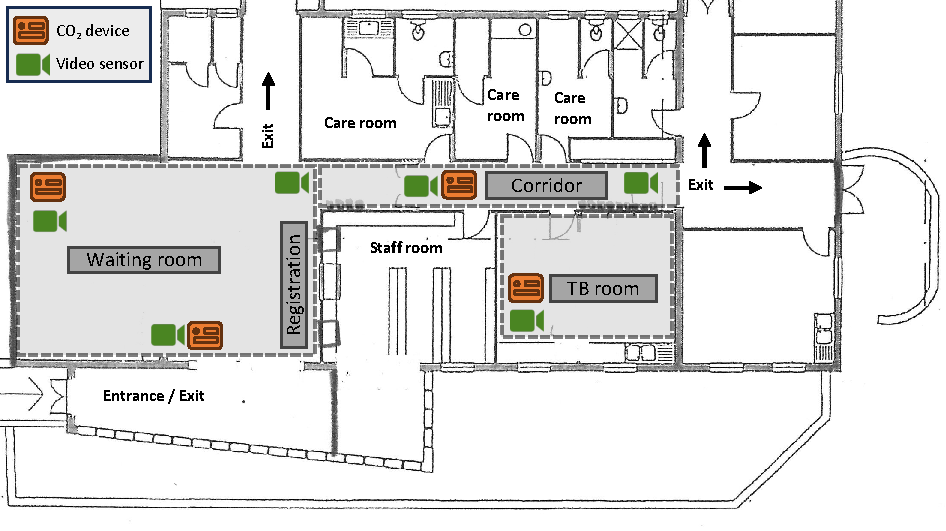
\includegraphics{doc/clinic-schematic-annotated-view.pdf}
    \caption{\textbf{Schematic view of the clinic}. Patients typically enter the clinic through the entrance on the bottom left, register at the reception, then wait in the waiting room or along the corridor until they see a doctor in one of the care rooms or the TB room, and finally exit the clinic through one of the exits in the waiting room or at the end of the corridor. Colored icons show the placement of the video sensors to track patient movements and the devices monitoring CO$_2$ levels.}
    \label{fig:floor-plan}
\end{figure}


\subsection{Data}

\subsubsection{Environmental data}

Four devices monitored indoor CO$_2$ levels (Digital CO$_2$ Monitor Carbon Dioxide Meter XE-2000, XEAST, Guangdong, China) in the waiting room, corridor, and TB room (\Cref{fig:floor-plan}). CO$_2$ levels were recorded in parts per million (ppm) at 1min intervals. Missing values were linearly imputed. On October~13, the corridor's CO$_2$ levels were missing and imputed with the waiting room's CO$_2$ levels because their CO$_2$ measurements were similar on the other days.    

\subsubsection{Clinical data}

We extracted clinical data from the electronic patient registry for all patients who attended the clinic during the study. Clinical records included the date and time of arrival, TB diagnostic results, and date of TB treatment initiation. We defined infectious patients as individuals who tested bacteriologically positive for TB during the study or who had received TB treatment for less than four weeks. Patients on treatment for more than four weeks or who had recently completed treatment were considered neither infectious nor susceptible. We also defined suspected TB patients as individuals who were tested for TB following symptom screening, but who were ultimately not diagnosed with TB. 

\subsubsection{Person tracking data}

We used an anonymous personal tracking system using video sensors (Xovis, Zollikofen, Switzerland) to monitor the movements of people (clinic staff, patients, and other visitors) throughout the clinic at 1~second intervals (\Cref{fig:floor-plan}). The resulting time-stamped tracking data consisted of a person’s height, their position recorded as x-y coordinates, and a unique ID for each person's track while in the clinic. \supp~Figure~\zref{fig:tracking-examples} shows some sample tracks from our study. Note that people in the clinic could contribute multiple tracks if they moved out of the range of a sensor or if they were briefly unrecognized as a person. To address these issues, we created an R Shiny tool to manually reconnect interrupted tracks back together (\supp~Text~\zref{sec:setting-and-data}). We also labeled the tracks to identify movements of the clinic staff.  

\subsection{The Wells-Riley equation}

Our spatiotemporal model is based on the Wells-Riley equation\cite{Riley1978AJE}, which estimates the risk (probability in \%) of infection $P$ as
\begin{align}
    P = \frac{D}{S} = 1 - \exp\left(\frac{Ipqt}{Q}\right),
\end{align}
where $D$ is the number of diseased cases, $S$ is the number of susceptible cases, $I$ is the number of infectious people in the indoor space, $p$ is the breathing rate (m$^3$ h$^{-1}$), $q$ is the quantum (infectious dose) generation rate (quanta h$^{-1}$), $t$ is the exposure time (h), and $Q$ is the ventilation rate (m$^3$ h$^{-1}$). The probability of infection is estimated with a Poisson relation, considering the stochastic behavior of airborne infection, where one quantum corresponds to a 67\% risk of infection. The main assumption of the Wells-Riley model is a well-mixed airspace, which means that the quanta concentration $N = Iq/Q$ (quanta m$^{-3}$) is the same everywhere in the room. Instead, our study considers a mixed airspace with spatial variation in the quanta concentration. This is accomplished using patient movement data combined with clinical records to identify the spatiotemporal location of infectious patients who generate quanta.

\subsection{Spatiotemporal modeling approach}

A detailed description of the Wells-Riley model and our spatiotemporal extension is provided in \supp~Text~\zref{sec:spattemp-model}. In the following, we describe the main components of our modeling approach, which are summarized in \Cref{fig:modeling-flow}.

\begin{figure}[!htpb]
    \centering
    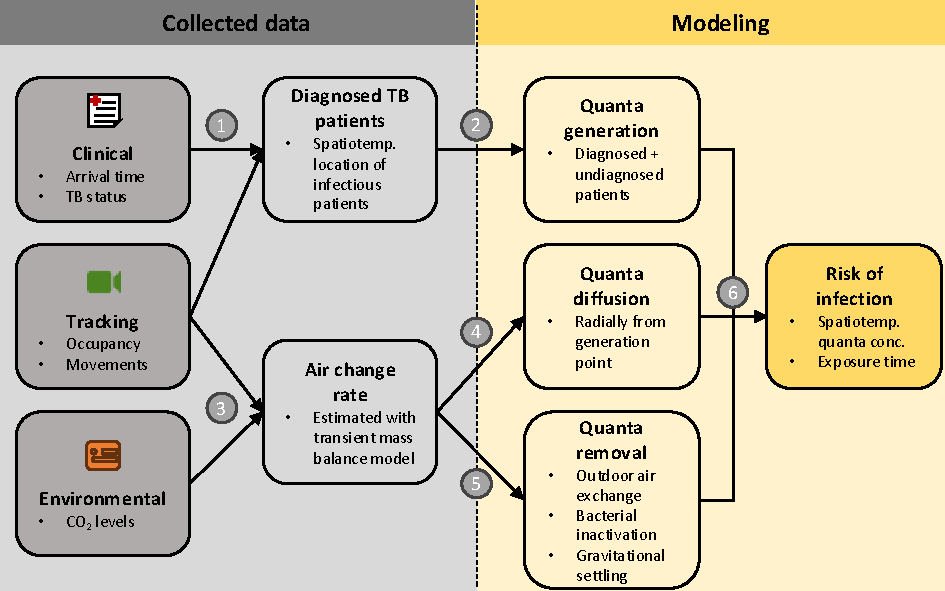
\includegraphics{doc/model-flow-chart.pdf}
    \caption{\textbf{Visual summary of the spatiotemporal modeling approach}. (1)~Clinical and person tracking data were combined to determine the spatiotemporal location of diagnosed (infectious) TB patients. (2)~Both diagnosed and randomly selected undiagnosed  TB among clinic attendees generate infectious quanta. (3)~Tracking and environmental data were combined to estimate the air change rate. (4)~Air change rate was related to the speed at which quanta diffuses indoors. (5)~The air change rate also determines quanta removal through outdoor air exchange, in addition to inactivation of \emph{Mtb} in airborne particles. (6)~Quanta generation, diffusion, and removal determine the spatiotemporal quanta concentration, from which the personal risk of infection is calculated using the Wells-Riley equation.}
    \label{fig:modeling-flow}
\end{figure}

\subsubsection*{Quanta generation}

(1)~We matched clinical and patient movement data to identify the spatiotemporal location of infectious TB patients within the clinic. We recorded the timestamp when the patient movement was detected in the registration area and matched this with the registration time in the clinical records. We excluded patient movements of less than five minutes and with less than five seconds in the registration area from the matching. Data were matched if there was a patient movement in the registration area followed by a entry in the clinical database, considering a maximum delay of 15 minutes. All diagnosed TB patients could be matched with patient movements this way. (2)~In addition to diagnosed TB patients, we also consider a number of undiagnosed (subclinical) TB patients. Prior studies suggest that the number of undiagnosed TB patients may be proportional to the number of diagnosed TB patients \cite{Berhanu2023CID,Moyo2022LancetID,Patterson2024PNAS}. Therefore, we model the number of undiagnosed TB patients with a multinomial distribution based on the counts of the daily number of diagnosed patients in the clinical data in October/November 2021 (\supp~Figure~\zref{fig:undiagnosed-distribution}): 6 days (12\%) with zero, 12 (41\%) with one, 8 (28\%) with two, 2 (7\%) with three, and 1 (3\%) with four TB patients visiting the clinic. Undiagnosed patients were randomly sampled among all clinic attendees with the same probability, excluding clinic staff who were not considered infectious. We further assumed that diagnosed and undiagnosed TB patients generated quantum at the same rate $q$, which was modeled using a lognormal prior distribution considering two different activity levels (\supp~Figure~\zref{fig:quanta-distribution}): median of 1.08\,quanta h$^{-1}$ (95\%-credible interval [CrI] 0.003\,quanta h$^{-1}$\,$-$\,386\,quanta h$^{-1}$) while sitting and 2.81\,quanta h$^{-1}$ (95\%-CrI 0.008\,quanta h$^{-1}$\,$-$\,987\,quanta h$^{-1}$) while walking\cite{Mikszewski2021GF,Buonanno2020EI,Banholzer2024PGPH}. Since mask wearing was mandatory for all clinic staff and attendees during the study, we assumed a mean reduction in $q$ by 75\% (95\%-CrI 56\%\,$-$\,86\%)\cite{Dharmadhikari2012AJRCCM,McCreesh2021BMJGlobalHealth}.

\subsubsection*{Quanta diffusion}

(3)~We calculated room occupancy from the video sensor data and combined it with the CO$_2$ measurements to estimate air change rates by daytime using a transient mass balance model\cite{Batterman2017IJERPH}. (4)~The air change rate was related to the diffusion of quanta using, as an approximation, the empirical relationship between the eddy diffusion coefficient and the air change rate in CO$_2$ particles\cite{Cheng2011EnvSciTech,Foat2020BE}. Since airflow was not monitored in our study, we assumed that the quanta diffused radially from where it had been generated (\supp~Figure~\zref{fig:toy-example}). 

\subsubsection*{Quanta removal}

(5)~Quanta removal occurs through replacement of contaminated indoor air with fresh outdoor air, inactivation of bacteria in airborne particles, and gravitational settling. The removal rate is thus the sum of the air change rate, the inactivation rate of \emph{Mtb}, and the gravitational settling rate. The bacterial inactivation rate of \emph{Mtb} was modeled using a lognormal prior distribution (\supp~Figure~\zref{fig:undiagnosed-distribution}) with a median of 1\,quanta h$^{-1}$ (95\%-CrI 0.1\,quanta h$^{-1}$\,$-$\,7.1\,quanta h$^{-1}$)\cite{Loudon1969AMRRD,Lever2000LettersAppliedMicrobio,Gannon2007ResVetSci,Klein2014IJMyco}. We set the gravitational settling rate to zero, thereby ignoring sedimentation because the particles carrying \emph{Mtb}, which are in the size range of $1-7\mu$m\cite{Fennelly2020Lancet}, are airborne immediately or within seconds\cite{Vuorinen2020SafSci}.

\subsubsection*{Risk of infection}

(6)~Based on the quanta generation, diffusion, and removal process, the quanta concentration $N$ (quanta\,m$^{-3}$) at time $t$ was computed as 
\begin{align}\label{eq:spattemp-N}
    \underbrace{N_{t}}_{\text{new concn.}} = \underbrace{\left(D \Delta (\underbrace{N_{t-1}}_{\text{prev. concn.}} + \underbrace{I_t \cdot q}_{\text{generation}})\right)}_{\text{diffusion}} \cdot \underbrace{\exp\left(-(AER_t + \lambda)\right)}_{\text{removal}} ~.
\end{align}
where $D$ is the diffusion constant (m$^2$ s$^{-1}$), $\Delta$ is the Laplace operator (second-order differential operator), $I_t$ is the number of infectious individuals in space, $q$ is the quantum generation rate (quanta\,s$^{-1}$), $AER$ is the air change rate (quanta\,s$^{-1}$), and $\lambda$ is bacterial inactivation rate (quanta\,s$^{-1}$). The patient-specific risk of infection depends on the cumulative exposure to infectious quanta and was computed using the Wells-Riley equation as
\begin{align}
    P = 1-\exp\left(-\sum_c \sum_t N_{c,t} \cdot \mathbb{I}_{c,t} \cdot p_a\right),
\end{align}
where $N_{c,t}$ is the quanta concentration in cell space $c$ at time $t$, $\mathbb{I}_{c,t}$ indicates whether the person was in $c$ at $t$, and $p_a$ (m$^3$ s$^{-1}$) is the breathing rate for activity level $a$. We distinguished between walking ($p_\mathrm{walk}$ = 1.33\,m$^3$ h$^{-1}$) and sitting activities ($p_\mathrm{sit}$ = 0.51\,m$^3$ h$^{-1}$)\cite{Adams1993}, based on whether the distance between two patient tracks was more or less than 0.25m.

\subsection{Monte Carlo simulation}

Our setup and simulation approach are described in detail in Text~\zref{sec:estimation}, including a comprehensive review of our modeling assumptions and choices of prior distributions. To summarize, we simulated the spatiotemporal quanta concentration separately for the waiting room, corridor, and TB room of the clinic. Each room was rasterized into a grid of cubic cells with a squared area of 0.25m$^2$. The quanta concentration was modeled during clinic hours from 8am to 4pm and updated every second. We used a Monte-Carlo simulation approach to consider uncertainty in key modeling parameters. In each simulation, we sampled uncertain modeling parameters from their prior distributions and, based on that, computed the spatiotemporal quanta concentration and the risk of infection per clinic attendee. 

\subsection{Hypothetical scenarios}

Our study was set during the COVID-19 pandemic when infection control measures were in place. To model their effectiveness, we considered two hypothetical scenarios: 1)~no mask wearing, \ie assuming no reduction in the quantum generation rate; and 2)~pre-pandemic ventilation conditions, \ie a fixed air change rate of 16 air changes per hour, corresponding to the average in our pre-pandemic pilot study in 2019\cite{Zurcher2022JID}. Furthermore, we examined the impact of different assumptions about the number of infectious patients in the clinic: 1)~instead of undiagnosed TB patients, we considered patients clinically suspected of having TB as infectious, because these patients may still generate aerosolized \emph{Mtb} even when they were not diagnosed with TB at first presentation\cite{Patterson2024PNAS}; 2)~randomly selecting infectious patients among all clinic attendees in proportion to the prevalence of TB in the South African population\cite{Moyo2022LancetID}, thereby pretending that the clinical data were not available. Except for the scenario-specific modifications, all other modeling assumptions and parameters were the same in each Monte Carlo simulation, ensuring comparability of the results. 

\subsection{Statistical analysis}

Clinical (diagnosed and suspected TB patients), environmental (time-varying CO$_2$ levels and air change rates), and patient movement data (spatiotemporal number of tracks, visit time, and close-contact encounters) were assessed descriptively and summarized with the median and interquartile range (IQR). Spatiotemporal quanta concentration and risk of infection per clinic attendee were estimated based on 5,000 Monte Carlo simulations. The average quanta concentration was computed by daytime (morning: 8am to 12am, afternoon: 12am to 4pm) and the risk of infection was summarized with the mean and 80\%-credible interval (CrI). A Bayesian Beta regression model was used to estimate the odds ratio (OR) of the modeled risk of TB infection in association with the visit time, duration of close contact, and frequency of close-contact encounters. All analyses were performed in R software (version 4.3.1) and the Bayesian regression model was estimated in the probabilistic programming language Stan (version 2.26.1).

\subsection{Ethics statement}

The University of Cape Town Faculty of Health Sciences Human Research Ethics Committee (HREC/REF: 228/2019), the City of Cape Town (Project ID: 8139), South Africa, and the Ethics Committee of the Canton of Bern (KEK/REF: 2019-02131), Switzerland, approved the study.

\newpage

\section{Results}

During one week corresponding to five open clinic days, 894 patients were registered in the clinical database, of whom four patients were bacteriologically diagnosed with TB and 16 patients were suspected of having TB after symptom screening (\supp~Figure~\zref{fig:diagnosed-tb-patients}). Overall, 1,563 unique movements were detected in the clinic after processing the video sensor data, of which 125 were labeled as healthcare worker, identifying 1,438 clinic attendees (patients or other visitors). Most movements were detected in the waiting room (\Cref{fig:input-data-descriptives}a) and during the morning (\Cref{fig:input-data-descriptives}b). Clinic attendees spent about half an hour in the clinic (median 25\,min, IQR 13\,min$-$46\,min), most of it in the waiting room (\Cref{fig:input-data-descriptives}c). Close-contact encounters (proximity <1\,m and duration >1\,min) were frequent (median 5, IQR 2$-$9) and clinic attendees were in close contact with at least one other person for more than half of their visit (median 68\%, IQR 41\%$-$87\%). The CO$_2$ levels in the clinic were low (median 431\,ppm, IQR 406\,ppm$-$458\,ppm (\supp~Figure~\zref{fig:co2-levels}) and the corresponding air change rates were high throughout the study (\Cref{fig:input-data-descriptives}g), with a \eg median of 29 air changes per hour (IQR 9\,h$^{-1}$$-$36\,h$^{-1}$) in the densely occupied waiting room. 


\begin{figure}
    \centering
     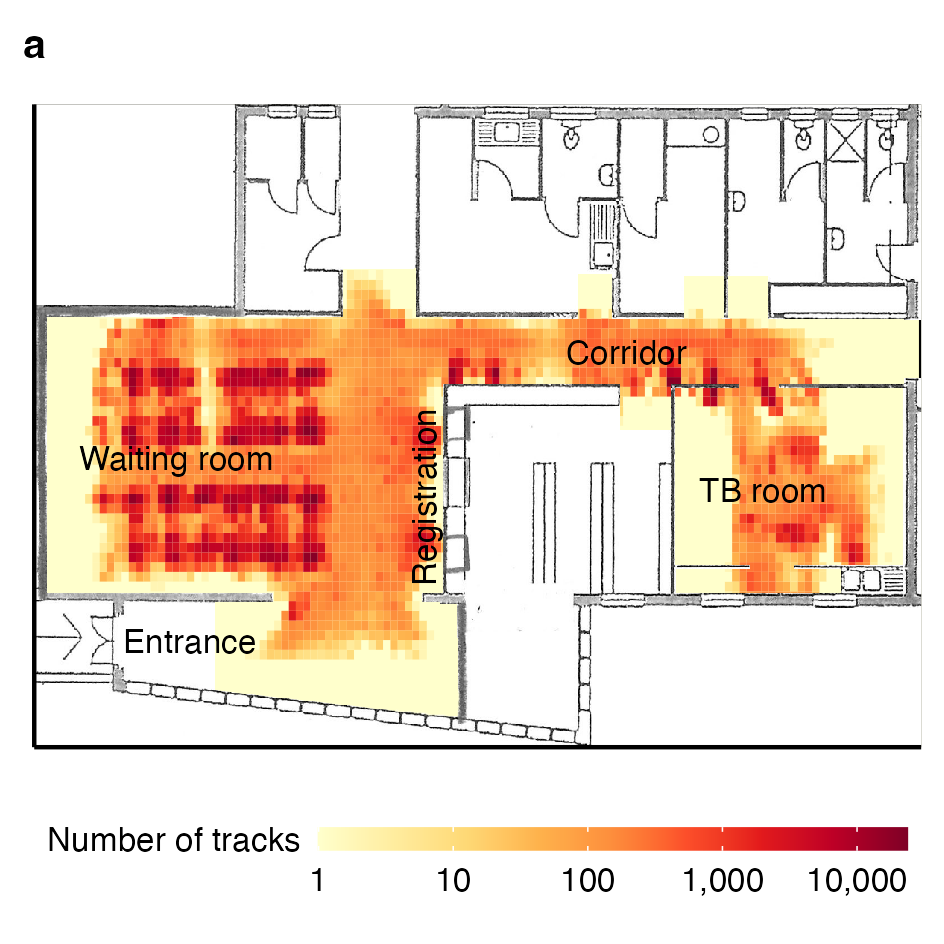
\includegraphics{results/data/no-people-spatial.png}
    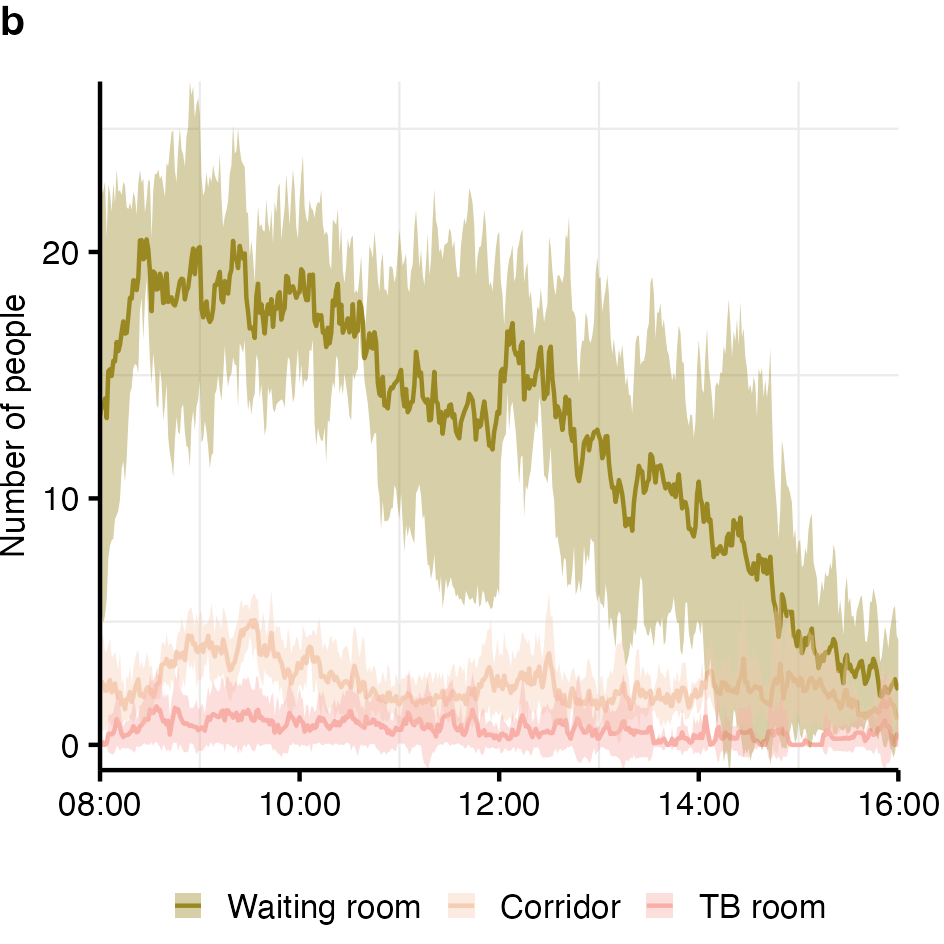
\includegraphics{results/data/no-people-over-time.png}
    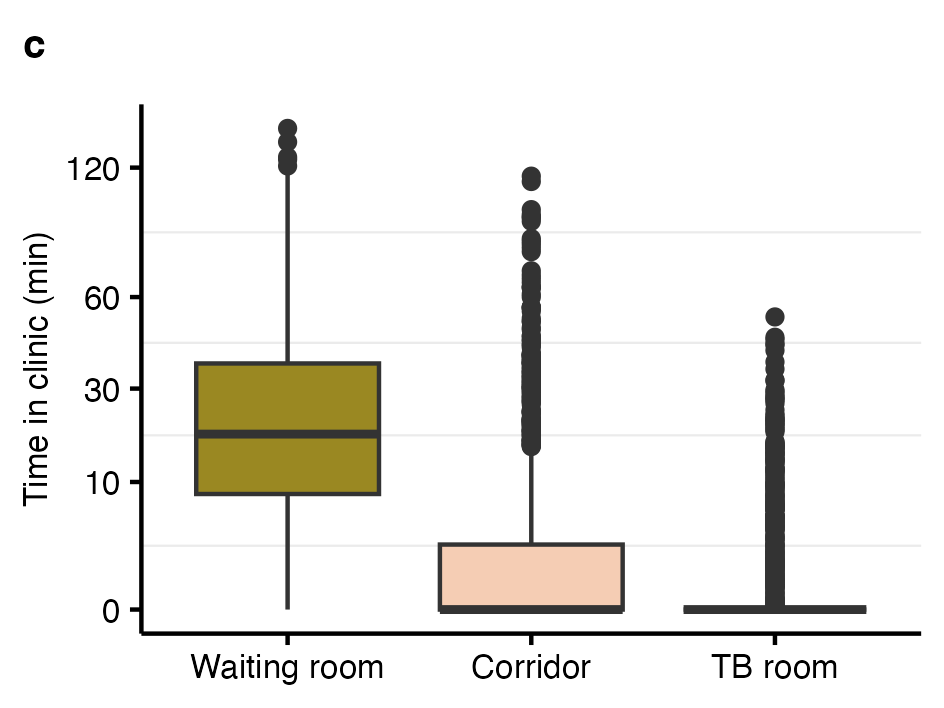
\includegraphics{results/data/time-in-clinic.png}
    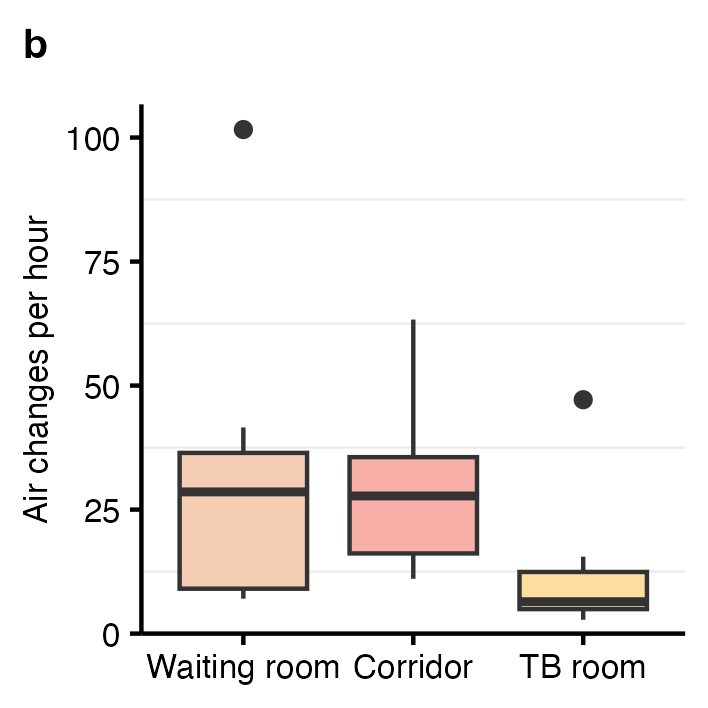
\includegraphics{results/data/air-changes-per-hour.png}
    \caption{\textbf{Patient movements and environmental conditions in the clinic.} Across clinic days and for the waiting room, corridor and TB room of the clinic: \textbf{(a)}~total number of tracks recorded per unit space, \textbf{(b)}~number of people in the clinic over time, \textbf{(c)}~time per clinic visit, and \textbf{(d)}~air change rates. Lines and ribbons show the mean plus/minus standard deviation, respectively. Boxplots show the median as lines, IQR as boxes, range as whiskers, and outliers as dots.}
    \label{fig:input-data-descriptives}
\end{figure}

\supp~File~1 shows an animated sequence of the spatiotemporally varying quanta concentration as an infectious patient enters the clinic on the morning of October 25 and moves through the waiting room. It can be seen that the quanta concentration was higher near the infectious patient, indicating his position and movement. The quanta diffused quickly because the diffusion constant was related to the air change rate, which was generally high because all doors and windows were typically open during clinic hours. Across clinic days, the quanta concentration was higher in the morning than in the afternoon, and higher in the waiting room than in the corridor or TB room of the clinic (\Cref{fig:main-modeling-results}). An exposure of one hour to the mean quanta concentration in the middle of the waiting room would correspond to a 0.21\% risk of infection in the morning compared to a 0.05\% risk in the afternoon. The mean risk of infection per clinic visit was 0.06\% (80\%-CrI 0.01\%$-$0.07\%), corresponding to a risk of 0.12\% per hour (80\%-CrI 0.01\%$-$0.23\%). To put this into perspective, a patient with twelve hourly visits per year would have a cumulative annual risk of infection of 1.37\% (80\%-CrI 0.14\%$-$2.74\%). 

Our modeling approach allowed us to estimate the individual risk of infection with uncertainty, for example, to identify patients with a comparably higher mean risk of infection and low uncertainty (\supp~Figure\zref{fig:patient-risk-focus}). The modeled individual risk of infection was further associated with the number of close contacts and the time spent in the clinic. When the number of close contacts doubled, the odds of infection increased to 1.17 (95\%-CrI 1.04$-$1.30). Similarly, doubling the time spent in the clinic increased the odds of infection to 1.09 (95\%-CrI 1.01$-$1.18). The time spent in close contact was not significantly associated with the individual risk of infection (1.05, 95\%-CrI, 0.96$-$1.14). Finally, a comparison of our spatiotemporal modeling results with those of a temporal model assuming a well-mixed airspace showed a notable difference in the individual risk of infection with a median of 8\% (IQR 4\%$-$15\%).  

\begin{figure}
    \centering
    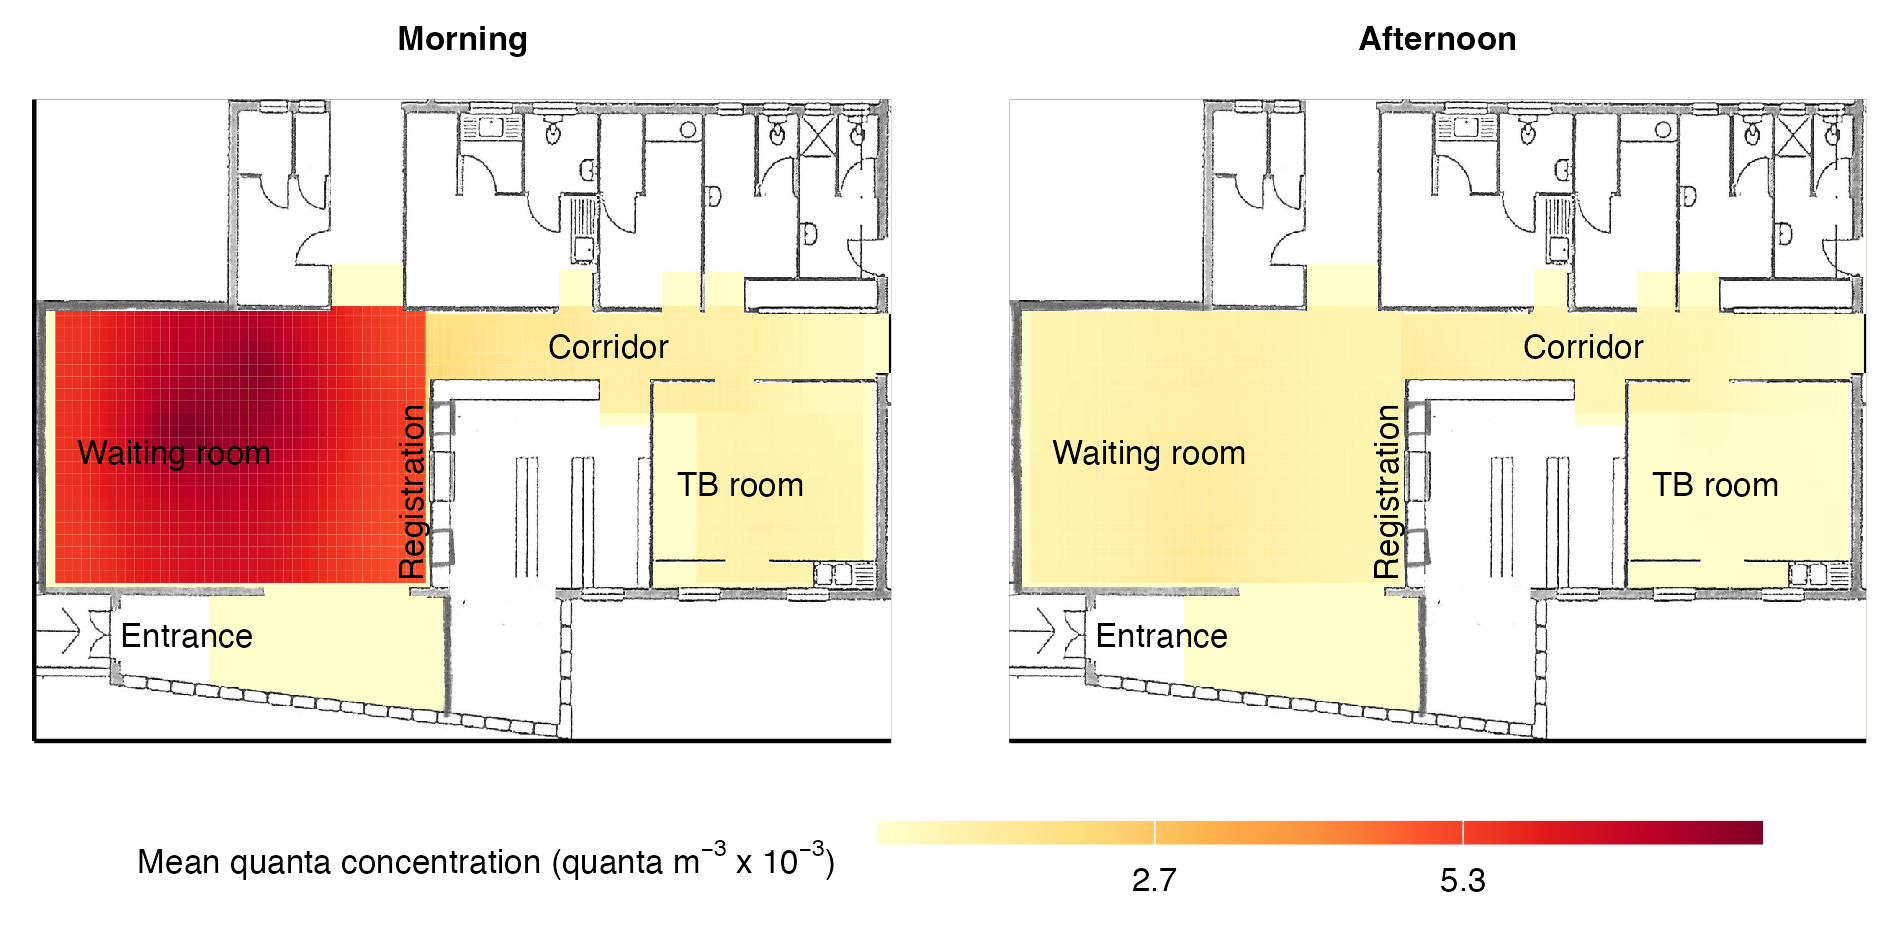
\includegraphics{results/modeling/mean-quanta-concentration.png}
    \caption{\textbf{Spatiotemporal quanta concentration in the clinic.} Model-estimated average quanta concentration across clinic days in the morning and afternoon in the waiting room, corridor and TB room of the clinic.}
    \label{fig:main-modeling-results}
\end{figure}

To assess the impact of infection control measures during the COVID-19 pandemic, we ran hypothetical scenarios assuming no mask use and pre-pandemic ventilation rates (\Cref{fig:scenario-results}). If none of the clinic attendees or staff had worn masks, the mean risk of infection per visit would have been 0.07\% (80\%-CrI 0.01\%$-$0.09\%), a 1.3-fold increase (80\%-CrI 1.2$-$1.4). If the air change rate had been the same as before the COVID-19 pandemic, the mean risk of infection would have been (0.10\%, 80\%-CrI 0.01\%$-$0.09\%), a 1.7-fold increase (80\%-CrI 0.5$-$5.3). Without mask use and with pre-pandemic ventilation rates, the mean risk of infection would have been (0.13\%, 95\%-CrI 0.01\%$-$0.13\%), a 2.5-fold increase (80\%-CrI 0.6$-$8.8). The scenarios show an increase in the number of clinic attendees with a high risk of infection, suggesting that universal use of mask and better ventilation in the clinic had a considerable impact on the tail of the risk distribution, which can also be seen in the smaller upper limit of the credible intervals. 

To assess the impact of modeling assumptions, we ran scenarios making different assumptions about the number of infectious people in the clinic. Assuming the number of infectious TB patients had been in proportion to the prevalence of TB in the South African population, the mean risk of infection would have been higher but the tail risk smaller (0.08\%, 80\%-CrI 0.02\%$-$0.13\%). Assuming that both diagnosed TB patients and clinic attendees suspected of TB infection had been infectious, both the mean and tail risk of infection would have been considerably higher (0.14\%, 80\%-CrI <0.01\%$-$0.26\%).  

\begin{figure}
    \centering
    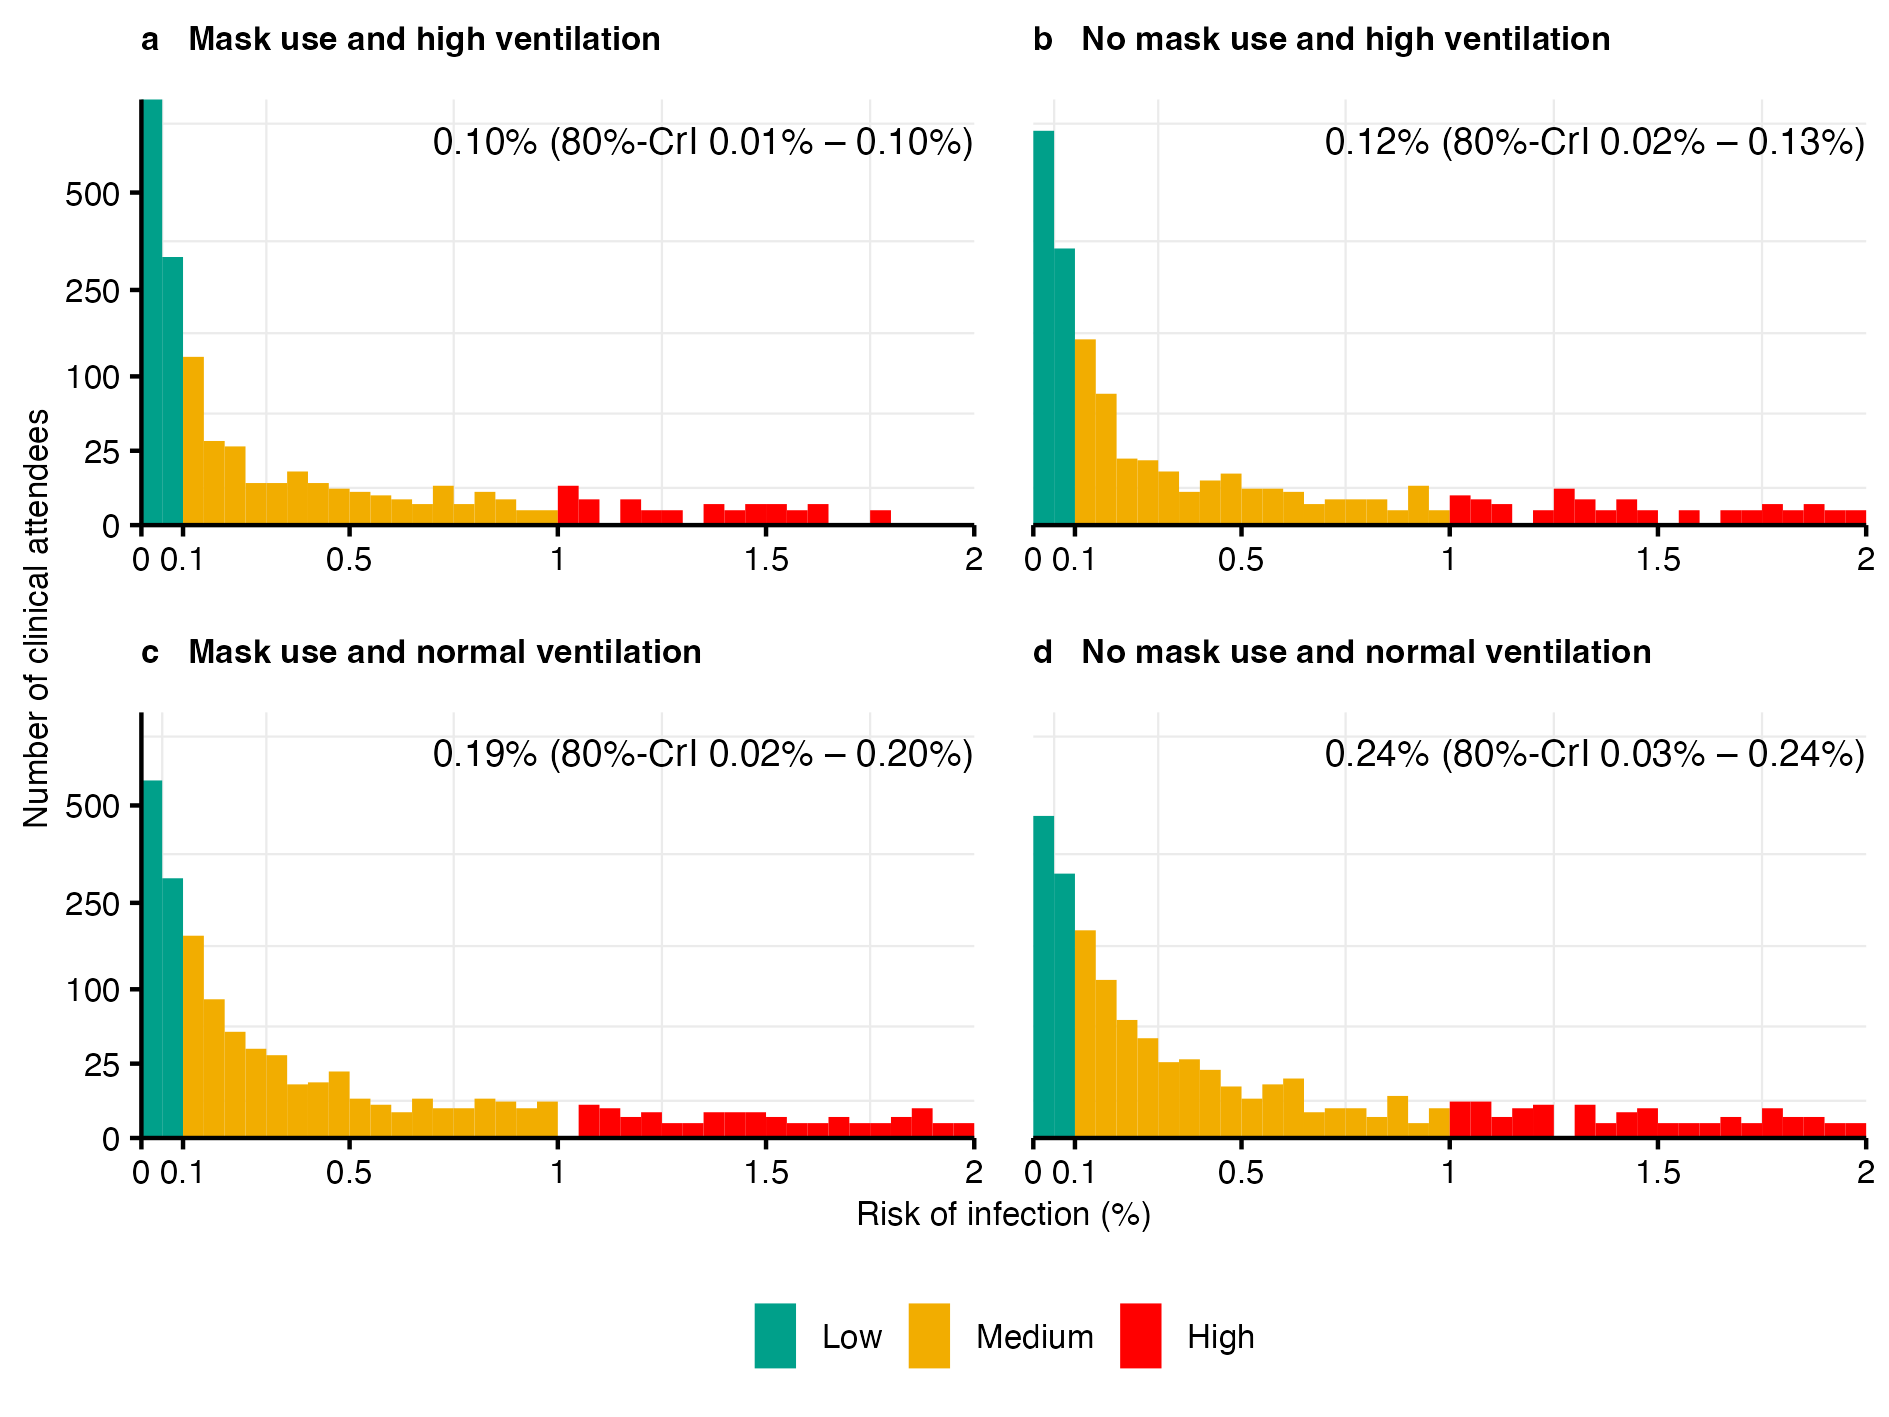
\includegraphics{results/modeling/mean-roi-comparison.png}
    \caption{\textbf{Impact of infection control measures.} Mean risk of infection per clinic visit: \textbf{(a)}~with mask use and high ventilation as experienced during the COVID-19 pandemic, \textbf{(b)}~without mask use and high ventilation, \textbf{(c)}~with mask use and normal ventilation as experienced before the COVID-19 pandemic  \textbf{(d)}~without mask use and normal ventilation. Low: <5\%, Medium: 5-10\%, High: >10\% risk of infection.}
    \label{fig:scenario-results}
\end{figure}


\FloatBarrier

\newpage

\section{Discussion}

% summary
We developed a spatiotemporal model to estimate the indoor concentration of infectious quanta and consider patient movement data from a South African primary care clinic in 2021 to accurately simulate the risk of Mtb infection for clinic attendees. We estimated an average risk of infection of 0.059\% (95\%-CrI 0.001\%$-$0.402\%), which would correspond to a cumulative annual risk of 0.7\% (95\%-CrI 0.01\%$-$4.72\%) if each patient visited the clinic once per month. Our model can identify patients with a higher risk of infection and low uncertainty. We also found that clinic attendees who stayed longer in the clinic and had more close-contact encounters  had a higher risk of infection, and we estimated the potential impact of infection control intervention. The modeled risk of infection would have been higher had infection control measures not been implemented during the COVID-19 pandemic such as compulsory face masks and improved ventilation conditions. Our spatiotemporal model can be readily adapted to model to other airborne transmission risk of other respiratory infections such as SARS-CoV-2.

% critical appraisal of our results
South Africa has a high burden of TB\cite{WHO2022TBReport}. Despite that, we estimated a low risk of infection per clinic attendee in our primary care clinic under pandemic conditions with strict infection control measures in place. In our previous pre-pandemic study before the COVID-19 pandemic, we estimated a cumulative annual risk of \emph{Mtb} transmission of between 9\% and 29\% for a patient coming to the clinic once per month for one hour. Although the assumed visit time is longer than what we observed in this study, the risk difference is still noteworthy and most likely due to the infection control measures that were in place during the SARS-CoV-2 pandemic. We estimated that without mask wearing or with pre-pandemic ventilation rates, the risk of infection would on average have been 1.28-fold or 1.74-fold higher, respectively. But mask wearing and natural ventilation were not the only measures in place during the pandemic, patient triage and fixed appointments probably also contributed to a further reduction in the risk of \emph{Mtb} transmission in our study. Finally, the risk difference could, to a small extent, be related to other factors. The risk estimate before the COVID-19 pandemic was based on TB prevalence in the South African population. We also estimated a higher mean risk of infection when modeling the risk based on TB prevalence or when considering both diagnosed and suspected TB patients as infectious. 

% relation to infection control
A previous modeling study estimated that between 4\% and 14\% of TB transmission in adults in a high TB burden, high HIV prevalence community in South Africa occurred in primary care clinics\cite{McCreesh2022BMJGlobalHealth}. Further studies suggest that compulsory face mask wearing could reduce the risk of \emph{Mtb} transmission by more than 50\%\cite{Dharmadhikari2012AJRCCM,McCreesh2021BMJGlobalHealth}. Our findings also suggest that the risk of infection is lower with mask wearing, although the risk reduction estimated in our study is less striking. The reason is that the effect of mask wearing is dominated by the impact of very high ventilation rates, which determine both the diffusion and removal of infectious quanta in the indoor space. The air change rates in the clinic typically ranged from 10 to 40 air changes per hour, which result in a quick diffusion and removal of infectious quanta from the indoor air. To put this into perspective, we recently modeled the risk of \emph{Mtb} transmission in schools comparing ventilation conditions in South Africa (1.48\,h$^{-1}$), Switzerland (0.71\,h$^{-1}$), and Tanzania (13.74\,h$^{-1}$)\cite{Banholzer2024PGPH}. Tanzania had a much lower estimated risk of \emph{Mtb} transmission in schools than the other countries, which was largely due to better ventilation, and yet its mean air change rate was less than half the rate measured in our study. Thus, we note that our study results do \emph{not} indicate that masks are less effective as found in other studies, rather their effectiveness is overshadowed by excellent ventilation conditions in the clinic during the COVID-19 pandemic.

% close contacts
Our spatiotemporal model can be viewed as a modified version of the Wells-Riley transmission model\cite{Riley1978AJE}, which assumes a well-mixed airspace. By contrast, our model allows the quanta concentration to vary both over time and space, considering that density of infectious particles is initially higher near the infectious source\cite{Wang2021Science,Vuorinen2020SafSci,Chen2020BuildEnv}. The exposure to infectious quanta therefore depends on the proximity to infectious individuals, which aligns with previous findings suggesting that prolonged close contact may be required for transmission of respiratory infections\cite{Leung2020NatMed,Brankston2007LancetID,Narasimhan2013PulmonaryMed}. In line with this, our modeled risk of infection was significantly associated with the number of close-contact encounters and the time spent in the clinic. This is because more close contacts and longer visits make exposure to high doses of infectious particles more likely. However, we note that this association is based on modeled results and it is difficult to definitively prove close contact respiratory transmission. Empirical studies investigating the potential link between contact data and respiratory transmission are so far scant\cite{Voirin2015ICHE,Vanhems2013PONE}.

% more complex models and our relation
Airborne respiratory transmission depends on common environmental and patient-specific factors.  Ventilation conditions and patient movements were considered by our model. However, other factors such as variation in infectiousness and susceptibility, temperature and humidity, or physiochemical properties of the infectious particles can further influence the generation, diffusion, and removal of infectious quanta (see \supp~Text~\zref{sec:depth-discussion} for a detailed discussion of these factors). For example, poor ventilation settings can impede the removal of infectious particles\cite{Li2021BuildEnv}, and computational fluid dynamics (CFD) models have been developed to consider airflow as an important factor influencing the spatial spread of airborne pathogens\cite{Vuorinen2020SafSci,Jung2021InfectChemo,Li2021BuildEnv,Yan2023BE,Qian2009BE,Li2022SOTTE}. However, CFD models are computationally expensive and primarily used in experimental settings and static environments, which makes their application to dynamic settings such as ours difficult. Moreover, our modeling approach necessitates computational efficiency because a large number of Monte Carlo simulations is required to reflect uncertainty in important modeling parameters. 

% limitations
Our modeling study has several limitations. First, tracking patient movements with video sensors is challenging and required considerable data processing and many patient movements were interrupted and could not be connected back together. Therefore, some clinic attendees may have had longer visits and the risk of infection may have been underestimated. Second, several important assumptions had to be made regarding the generation, diffusion, and removal of infectious quanta. Uncertainty in these modeling parameters was often large and could potentially be reduced in future workby incorporating , for example, additional information on patient characteristics from clinical records that are known to be associated with patient-specific infectiousness\cite{Escombe2008PLoSMed} or susceptibility\cite{Furin2019Lancet}. Third, we could not validate our modeling results with empirical findings. Future research could test the practical implementation of our model by examining whether clinic attendees with a high risk of infection were also subsequently more likely to be infected.  

% conclusions
In conclusion, our novel spatio-temporal transmission model study using clinical, environmental, and patient movement data showed that the risk of \emph{Mtb} transmission in a primary care clinic in South Africa under pandemic conditions with strict infection control measures in place.  The modeled risk of infection was significantly associated with the number of close-contact encounters by clinic attendees during their visit. Our spatiotemporal model could thus be used to assess the impact of interventions targeting patient flows that aim to reduce the number of close-contact encounters. 


\newpage


%TC:ignore
\section*{Acknowledgements}
...

\bibliography{references.bib}
%TC:endignore

\end{document}
